% Search for all the places that say "PUT SOMETHING HERE".

\documentclass[11pt]{article}
\usepackage{textcomp,graphicx,enumerate}
\usepackage[utf8]{inputenc}
\usepackage[english]{babel}
\usepackage{amsthm}
\usepackage{proof}
\usepackage{diagbox}
\usepackage{algorithmicx}  
\usepackage{subcaption}
\def\Name{Yingkun Zhou}  % Your name
\def\Email{zhouyingkun15@mails.ucas.ac.cn}
\title{Chisel Tutorial read note}
\author{\Name \\ \Email}
\pagestyle{myheadings}
\newtheorem*{remark}{Remark}
\newenvironment{qparts}{\begin{enumerate}[{(}a{)}]}{\end{enumerate}}
\def\endproofmark{$\Box$}

\textheight=9in
\textwidth=6.5in
\topmargin=-.75in
\oddsidemargin=0.25in
\evensidemargin=0.25in
\usepackage[procnames]{listings}
\usepackage[T1]{fontenc}
\usepackage{beramono}
\usepackage{listings}
\usepackage{xcolor}
\usepackage{hyperref}
\hypersetup{
	colorlinks=true,
	linkcolor=blue,
	filecolor=magenta,      
	urlcolor=cyan,
}

\definecolor{dkgreen}{rgb}{0,0.6,0}
\definecolor{gray}{rgb}{0.5,0.5,0.5}
\definecolor{mauve}{rgb}{0.58,0,0.82}

\lstdefinestyle{myScalastyle}{
	frame=tb,
	language=scala,
	aboveskip=3mm,
	belowskip=3mm,
	showstringspaces=false,
	columns=flexible,
	basicstyle={\small\ttfamily},
	numbers=none,
	numberstyle=\tiny\color{gray},
	keywordstyle=\color{blue},
	commentstyle=\color{dkgreen},
	stringstyle=\color{mauve},
	frame=single,
	breaklines=true,
	breakatwhitespace=true,
	tabsize=3,
}
\usepackage{amssymb} % needed for math
\usepackage{amsmath} % needed for math
\usepackage[utf8]{inputenc} % this is needed for german umlauts
\usepackage[T1]{fontenc}    % this is needed for correct output of umlauts in pdf
\usepackage[margin=2.5cm]{geometry} %layout
\usepackage{listings} % needed for the inclusion of source code

% the following is needed for syntax highlighting
\usepackage{color}
\definecolor{keywords}{RGB}{255,0,90}
\definecolor{comments}{RGB}{0,0,113}
\definecolor{red}{RGB}{160,0,0}
\definecolor{green}{RGB}{0,150,0}
\makeatletter
\newcommand{\rmnum}[1]{\romannumeral #1}
\newcommand{\Rmnum}[1]{\expandafter\@slowromancap\romannumeral #1@}
\makeatother
\lstset{language=Python, 
	basicstyle=\ttfamily\small, 
	keywordstyle=\color{keywords},
	commentstyle=\color{comments},
	stringstyle=\color{red},
	showstringspaces=false,
	identifierstyle=\color{green},
	procnamekeys={def,class}}

% this is needed for forms and links within the text
\usepackage{hyperref}
\newcommand{\note}[1]{\scriptsize{#1}\normalsize}
\newcommand{\emphasize}[1]{\huge{#1}\normalsize}
\begin{document}
\maketitle
\section*{1.Introduce}
\textbf{What is chisel?}

Chisel is really only a set of special class definitions, predefined objects, and usage conventions within Scala, so when you write a Chisel program you are actually writing a Scala program.

\textbf{The main goal of the tutorial}

The tutorial says that significant hardware designs can be completed using only the material contained herein.

\textbf{The motivation of chisel}

The team of chisel were motivated to develop a new hardware language by yeas of struggle e with existing hardware description languages in our research projects and hardware design courses. Verilog and VHDL were developed as hardware simulation languages, and only later did they become a basis for hardware synthesis. Much of the semantics of these languages are
not appropriate for hardware synthesis and, in fact,
many constructs are simply not synthesizable. Other
constructs are non-intuitive in how they map to hardware implementations, or their use can accidently lead
to highly inefficient hardware structures. While it is
possible to use a subset of these languages and yield
acceptable results, they nonetheless present a cluttered
and confusing specification model, particularly in an
instructional setting.

\textbf{Disadvantage of Verilog and VHDL}

While Verilog and VHDL include some
primitive constructs for programmatic circuit generation, they lack the powerful facilities present in modern programming languages, such as object-oriented
programming, type inference, support for functional
programming, and reflection.

\textbf{Why Scala}

picked Scala not only because it includes the programming features we feel are important for building circuit generators, but because it was specifically developed as a base for domain-specific languages.
\section*{2.Hardware expressible in Chisel}
\textbf{The basic model}

The initial version of Chisel only supports the expression of synchronous RTL (Register-Transfer Level)
designs, with a single common clock. Synchronous
RTL circuits can be expressed as a hierarchical composition of modules containing combinational logic
and clocked state elements. Although Chisel assumes
a single global clock, local clock gating logic is automatically generated for every state element in the
design to save power.
\begin{remark}
	Modern hardware designs often include multiple islands of logic, where each island uses a different clock
	and where islands must correctly communicate across
	clock island boundaries. Although clock-crossing synchronization circuits are notoriously difficult to design, there are known good solutions for most scenarios, which can be packaged as library elements for use
	by designers. As a result, most effort in new designs
	is spent in developing and verifying the functionality within each synchronous island rather than on
	passing values between islands.
\end{remark}

\section*{3.Datatypes in Chisel}
\begin{itemize}
	\item SInt
	\item UInt
	\item Bool
	\item Bundles (similar to structs in other languages)
	\item Vecs (for indexable collections of values)
\end{itemize}

\section*{4.Combinational Circuits}
\textbf{basic model}

A circuit is represented as a graph of nodes in Chisel. Each node is a hardware operator that has \textbf{zero or more} inputs and that drives \textbf{one} output.

The direct way is converting expression into a circuit tree, with named wires at the leaves and operators forming the internal nodes. But the more efficient circuit is in the shape of DAGs.

\section*{5.Builtin Operators}
\textbf{Bitwidth Inference}
Bit-width inference process will converge to a fixpoint
The width of a register must be specified by the user either explicitly or from the bitwidth of the reset value or the next parameter.

We have to use triple equals === for equality and =/= for inequality to allow the native Scala equals operator to remain usable.

\section*{6.Functional Abstraction}
\textbf{function invoke}

zero or more input and one output like the following example
\begin{lstlisting}[style=myScalastyle]
val out = clb(a,b,c,d)
\end{lstlisting}
\textbf{function definition}

in order to do that, we must define the function which takes a,b,c,d as arguments and returns a wire to the output of a boolean circuit.
\begin{lstlisting}[style=myScalastyle]
def clb(a: UInt, b: UInt, c: UInt, d: UInt): UInt = 
	(a & b) | (~c & d)
\end{lstlisting}
\section*{7.Bundles and Vecs(aggregate classes)}
well, it seems like that Vecs are kind of reg array.

after all, the superclass of all is data
\begin{remark}[1]
	Bundles and Vecs can be arbitrarily nested to build complex data structures
\end{remark}
\begin{remark}[2]
	the builtin Chisel primitive and aggregate classes do not require the new when creating an instance, whereas new user datatypes will, but not always stand.
\end{remark}

\section*{8.Ports}
Here is the example:
\begin{lstlisting}[style=myScalastyle]
	class Decoupled extends Bundle {
		val ready = Output(Bool())
		val data = Input(UInt(32.W))
		val valid = Input(Bool())
	}
\end{lstlisting}
which is a standard shackhand port type

also the port can use user defined class. In other words, folding directions into the object declarations.
\begin{lstlisting}[style = myScalastyle]
	class ScaleIO extends Bundle {
		val in = new MyFloat().asInput
		val scale = new MyFloat().asInput
		val out = new MyFloat().asOutput
	}
\end{lstlisting}
the methods asInput and asOutput force all modules of the data object to the requested direction.
\section*{9.Modules}

The hierarchical module namespace is accessible in downstream tools to aid in debugging and physical layout. A user-defined module is defined as a class
\begin{lstlisting}[style = myScalastyle]
	class Mux2 extends Module {
		val io = IO(new Bundle{
			val sel = Input(UInt(1.W))
			val in0 = Input(UInt(1.W))
			val in1 = Input(UInt(1.W))
			val out = Output(UInt(1.W))
		})
		io.out := (io.sel & io.in1) | (~io.sel & io.in0)
	}
\end{lstlisting}

\begin{remark}
	The := assignment operator, used here in the body of the definition, is a special operator in Chisel that wires the input of left-hand side to the output of the right-hand side
\end{remark}

\textbf{module constructor function invoke}

\begin{lstlisting}[style = myScalastyle]
val m1 = Module(new Mux2())
\end{lstlisting}

\section*{10.running examples and test them}
\begin{itemize}
	\item \textbf{poke} to set input port and state values
	\item \textbf{step} to execute the circuit one time unit
	\item \textbf{peek} to read port and state values
	\item \textbf{expect} to compare peeked circuit values to expected arguments
\end{itemize}
\begin{remark}
	Chisel produces Firrtl intermediate representation
	(IR). Firrtl can be interpreted directly or can be
	translated into Verilog, which can then be used to
	generate a C++ simulator through verilator.
\end{remark}
\textbf{To do this,
	on each iteration we generate appropriate inputs to
	the module and tell the simulation to assign these
	values to the inputs of the device we are testing (module or class) c,
	step the circuit 1 clock cycle, and test the expected
	value. Steps are necessary to update registers and
	the combinational logic driven by registers. For pure
	combinational paths, poke alone is sufficient to up-
	date all combinational paths connected to the poked
	input wire.
}
\begin{remark}
	For sequential modules we may want to delay the output definition to the appropriate time as the step function implicitly advances the clock one period in the simulation. Unlike Verilog, you do not need to explicitly specify the timing advances of the simulation; Chisel will take care of these details for you.
\end{remark}
what will happen in testing. By default, it will run the tests defined simulated but the Firrtl interpreter. We can instead have the module be simulated by a C++ simulator generated by Verilator by explicit typing verilator 

\section*{11.State Elements}
The simplest form of state element supported by Chisel is a positive edge-triggered register.
\begin{lstlisting}[style = myScalastyle]
val reg = Reg(next = in)
\end{lstlisting}
if you think about it carefully, the state element (here I mean single variable) has two faces: one is the input and one is the output. And the output is the copy of the input signal in delayed by one clock cycle.
\begin{remark}[1]
	we do not have to specify the type of Reg as it will be automatically inferred from its input when instantiated in
	this way.
\end{remark}
\begin{remark}[2]
	In the current version of Chisel, clock and
	reset are global signals that are implicitly included
	where needed
\end{remark}
\begin{remark}[3]
	the := assignment to variable say x wires an update combinational circuit on the right hand side(rhs) to the target node on the left hand side(lhs). As for reg associate circuit, the rule means that when x appears on the rhs of an assignment, its output is referenced, whereas when on lhs, its input is referenced.
\end{remark}
\begin{remark}[4]
	Purely combinational circuits cannot have cycles be-
	tween nodes, and Chisel will report an error if sucha cycle is detected. Just as said before, the pure combinational circuits is a DAG. Because they do not have cycles, combinational circuit can always be constructed in a feed-forward manner. \textbf{However}, sequential circuits naturally have feedback between nodes, and so it is sometimes necessary to reference an output wire before the producing node has defined.
	\begin{lstlisting}[style = myScalastyle]
	val pcPlus4 = UInt()
	val brTarget = UInt()
	val pcNext = Mux(io.ctrl.pcSel, brTarget, pcPlus4)
	val pcReg = Reg(next = pcNext, init = 0.U(32.W))
	pcPlus4 := pcReg + 4.U
	...
	brTarget :=	addOut
	\end{lstlisting}
\end{remark}
\begin{remark}[5]
	In a sequence of conditional updates, the last conditional update whose condition is true takes priority. the circuit is look like following:
	\begin{center}
		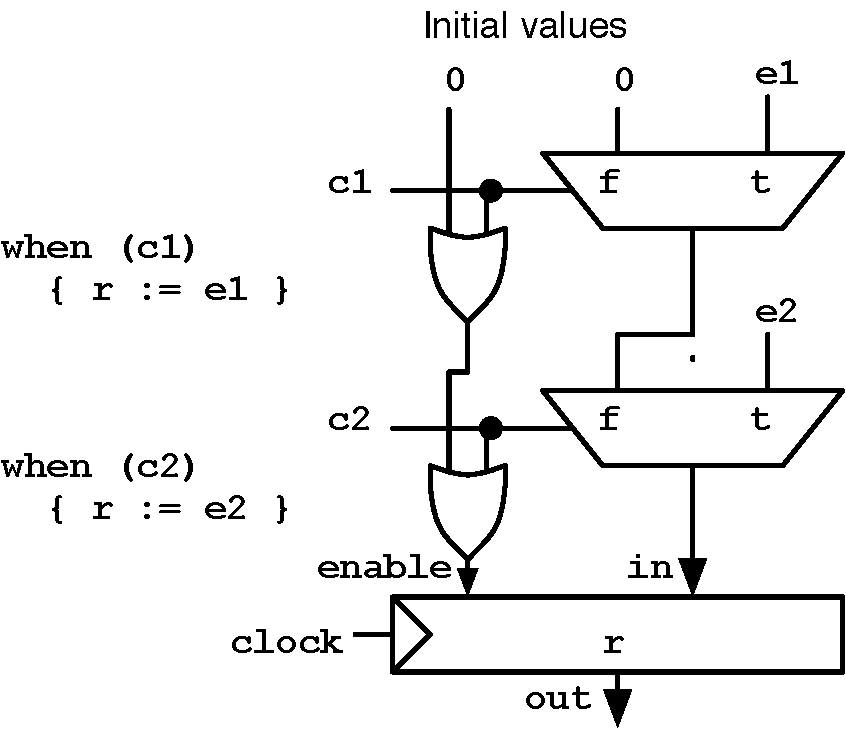
\includegraphics[width=\linewidth/2]{condupdates.pdf}
	\end{center}
	Each when statement adds anotherlevel of data mux and ORs the predicate into the enable chain. The compiler effectively adds the termination values to the end of the chain automatically
\end{remark}
\begin{remark}
	considering update of a wire. Note that all combinational circuits need a default value.
\end{remark}

\section*{Memories}
At most of time, we only care about SRAM. Here are two type SRAMs
\begin{lstlisting}[style = myScalastyle]
//A one-read port, one-write port SRAM
val ram1r1w =
	Mem(1024, UInt(32.W))
val reg_raddr = Reg(UInt())
when (wen) { ram1r1w(waddr) := wdata }
when (ren) { reg_raddr := raddr }
val rdata = ram1r1w(reg_raddr)
\end{lstlisting}
\begin{lstlisting}[style = myScalastyle]
//Single-ported SRAMs read and write conditions are mutually exclusive in the same when chain and write first.
val ram1p = Mem(1024, UInt(32.W))
val reg_raddr = Reg(UInt())
when (wen) { ram1p(waddr) := wdata }
.elsewhen (ren) { reg_raddr := raddr }
val rdata = ram1p(reg_raddr)
\end{lstlisting}
\begin{remark}
	Note that when constructing a memory in Chisel, the initial value of memory contents cannot be specified. Therefore, you should never assume anything about the initial contents of your Mem class.
\end{remark}

\section*{13.Interfaces \& Bulk Connections}
The ports in chisel support Subclasses and Nesting, which benefits code reuse.
\begin{lstlisting}[style = myScalastyle]
class SimpleLink extends Bundle { 
	val data  = Output(UInt(16.W)) 
	val valid = Output(Bool())
}

class PLink extends SimpleLink { 
	val parity = Output(UInt(5.W)) 
}

class FilterIO extends Bundle { 
	val x = new PLink().flip() //???
	val y = new PLink()
}

class Filter extends Module { 
	val io = IO(new FilterIO())
	...
}
\end{lstlisting}

\textbf{Bulk Connections}
\begin{lstlisting}[style = myScalastyle]
class Block extends Module { 
	val io = IO(new FilterIO())
	val f1 = Module(new Filter())
	val f2 = Module(new Filter())

	f1.io.x <> io.x
	f1.io.y <> f2.io.x
	f2.io.y <> io.y
}
\end{lstlisting}
in the above way, we can compose two filters into a filter block as follows

\section*{14.Functional Module Creation}
\begin{lstlisting}[style = myScalastyle]
object Mux2 {
	def apply (sel: UInt, in0: UInt, in1: UInt) = {
		val m = new Mux2()
		m.io.in0 := in0
		m.io.in1 := in1
		m.io.sel := sel
		m.io.out
	}
}


class Mux4 extends Module {
	val io = IO(new Bundle {
		val in0 = Input(UInt(1.W))
		val in1 = Input(UInt(1.W))
		val in2 = Input(UInt(1.W))
		val in3 = Input(UInt(1.W))
		val sel = Input(UInt(2.W))
		val out = Output(UInt(1.W))
	})
	io.out := Mux2(io.sel(1),
	Mux2(io.sel(0), io.in0, io.in1),
	Mux2(io.sel(0), io.in2, io.in3))
}
\end{lstlisting}
Selecting inputs is so useful
\begin{lstlisting}[style = myScalastyle]
Mux(c1, a, Mux(c2, b, Mux(..., default)))
MuxCase(default, Array(c1 -> a, c2 -> b, ...))
MuxCase(default, 
			  Array((idx === 0.U) -> a,
			    		 (idx === 1.U) -> b, ...))
MuxLookup(idx, default, 
				 Array(0.U -> a, 1.U -> b, ...))
\end{lstlisting}
\begin{remark}
	the cases (eg. c1,c2) must be in parentheses.
\end{remark}

\section*{15.Polymorphism and Parameterization}
\textbf{Parameterized Functions}

consider the following function:
\[ y[t] = \sum_{j} w_j * x[t - j] \]
\begin{lstlisting}[style = myScalastyle]
def Delays[T <: Data](x: T, n: Int): List[T] = 
	if (n <= 1) List(x) else x :: Delays(RegNext(x), n-1)

def FIR[T <: Data with Num[T]](w: Seq[T], x: T): T = 
	(w, Delays(x, w.length)).zipped.map(_ * _).reduce(_ + _)
\end{lstlisting}
explanation:
where delays creates a list of incrementally increasing delays of its input and reduce constructs a reduction circuit given a binary combiner function f. In this case, reduce creates a summation circuit. Finally, the FIR function is constrained to work on inputs of type Num where Chisel multiplication and addition are defined.

Somehow, the circuit logic can also write in this way:
\begin{lstlisting}[style = myScalastyle]
def Delay[T <: Bits](x: T, n: Int): T = 
	if (n == 0) x else Reg(Delay(x, n - 1))

def FIR[T <: Num] (w: Array[Int], x: T) = {
	val delays = Range(0, w.length).map(i => Num(w(i)) * Delay(x, i)
	delays.foldRight(_ + _)
}
\end{lstlisting}

\textbf{Parameterized Classes}
Like parameterized functions, we can parameterize classes to make them more reusable. For instance:
\begin{lstlisting}[style = myScalastyle]
class FilterIO[T <: Data](type: T) extends Bundle { 
	val x = type.asInput.flip // filp() ???
	val y = type.asOutput
}

class Filter[T <: Data](type: T) extends Module { 
	val io = IO(new FilterIO(type))
	...
}

val f = Module(new Filter(new PLink()))
\end{lstlisting}
another very useful example is fifo
\begin{lstlisting}[style = myScalastyle]
class DataBundle extends Bundle {
	val A = UInt(32.W)
	val B = UInt(32.W)
}

object FifoDemo {
	def apply () = new Fifo(new DataBundle, 32)
}

class Fifo[T <: Data] (type: T, n: Int) extends Module {
	val io = IO(new Bundle {
		val enq_val = Input(Bool())
		val enq_rdy = Output(Bool())
		val deq_val = Output(Bool())
		val deq_rdy = Input(Bool())
		val enq_dat = type.asInput
		val deq_dat = type.asOutput
	})
	val enq_ptr      = Reg(init = 0.U(sizeof(n).W))
	val deq_ptr      = Reg(init = 0.U(sizeof(n).W))
	val is_full      = Reg(init = false.B)
	val do_enq       = io.enq_rdy && io.enq_val
	val do_deq       = io.deq_rdy && io.deq_val
	val is_empty     = !is_full && (enq_ptr === deq_ptr)
	val deq_ptr_inc  = deq_ptr + 1.U
	val enq_ptr_inc  = enq_ptr + 1.U
	val is_full_next = 
	Mux(do_enq && ~do_deq && (enq_ptr_inc === deq_ptr), 
	true.B,
	Mux(do_deq && is_full, false.B, is_full))
	enq_ptr := Mux(do_enq, enq_ptr_inc, enq_ptr)
	deq_ptr := Mux(do_deq, deq_ptr_inc, deq_ptr)
	is_full := is_full_next
	val ram = Mem(n)
	when (do_enq) {
		ram(enq_ptr) := io.enq_dat
	}
	io.enq_rdy := !is_full
	io.deq_val := !is_empty
	ram(deq_ptr) <> io.deq_dat
}
\end{lstlisting}

It is also possible to define a generic decoupled interface:
\begin{lstlisting}[style = myScalastyle]
class DecoupledIO[T <: Data](data: T) 
    extends Bundle {
  val ready = Input(Bool())
  val valid = Output(Bool())
  val data  = data.cloneType.asOutput
}

class DecoupledDemo 
  extends DecoupledIO()( new DataBundle ) //????

class Fifo[T <: Data] (data: T, n: Int) 
    extends Module {
  val io = IO(new Bundle {
    val enq = new DecoupledIO( data ).flip()
    val deq = new DecoupledIO( data )
  })
  ...
}
\end{lstlisting}
\section*{16.further reading about chisel}
\begin{itemize}
	\item the tool that can translate
	the first implemented RISC-V processor  \href{https://github.com/aswaterman/trainwreck}{trainwreck}
	\item What's the difference between chisel 2 and chisel 3
	\href{https://github.com/freechipsproject/chisel3/wiki/Chisel3-vs-Chisel2}{Chisel3 vs Chisel2}
	\item  useful \href{https://github.com/freechipsproject/chisel3/wiki}{wiki} and \href{https://github.com/ucb-bar/chisel-tutorial/wiki}{tutorial} to introduce Chisel
	\item \href{https://docs.scala-lang.org/tour/tour-of-scala.html}{tour of scala}
\end{itemize}
 
\end{document}

